\documentclass[12pt,a4paper]{report}
\usepackage{color}
\usepackage{amsmath}
\usepackage{graphicx}
\usepackage{upquote}
\newcommand{\blank}[1]{\hspace*{#1}}
\usepackage{setspace}
%\onehalfspacing
\doublespacing
\newcommand*{\rom}[1]{\expandafter\@slowromancap\romannumeral #1@}
\makeatother
\usepackage{fancyhdr}




    \pagestyle{fancy}
\usepackage{blindtext}

\lhead{\footnotesize{Bitcoin: A Peer-to-Peer Electronic Cash System}}
\chead{}
\rhead{}
\lfoot{\footnotesize{Department of ECE, PESIT-BSC }}
\cfoot{}
\rfoot{Page \thepage}
\renewcommand{\headrulewidth}{1pt}
\renewcommand{\footrulewidth}{1pt}
%\footnotetext{Department of ECE, PESIT-BSC  \blank{6cm}}




\usepackage
[
        a4paper,% other options: a3paper, a5paper, etc
        left=1.25in,
        right=1in,
        top=0.75in,
        bottom=0.75in,
        % use vmargin=2cm to make vertical margins equal to 2cm.
        % us  hmargin=3cm to make horizontal margins equal to 3cm.
        % use margin=3cm to make all margins  equal to 3cm.
]
{geometry}
\usepackage{lipsum}
\usepackage{multirow}
\pagenumbering{roman}
\usepackage{pgf}
\usepackage{pgfpages}
\pgfpagesdeclarelayout{boxed}
{
  \edef\pgfpageoptionborder{0pt}
}
{
  \pgfpagesphysicalpageoptions
  {%
    logical pages=1,%
  }
  \pgfpageslogicalpageoptions{1}
  {
    border code=\pgfsetlinewidth{2pt}\pgfstroke,%
    border shrink=\pgfpageoptionborder,%
    resized width=.95\pgfphysicalwidth,%
    resized height=.95\pgfphysicalheight,%
    center=\pgfpoint{.5\pgfphysicalwidth}{.5\pgfphysicalheight}%
  }%
}
\pgfpagesuselayout{boxed}

\begin{document}
%\setcounter{page}{i}
\begin{center}\underline{ \Large\textbf{ACKNOWLEDGEMENT}}\end{center}
It is always a pleasure to remind the faculty of PESIT-BSC for their sincere guidance and support to intensify my wisdom and give me the opportunity to present what I have learned. I would like to thank to my parents for the encouragement, enthusiasm and invaluable lessons given, which have ingrained in me a sense of curiosity and wonder to attain an unquenchable thirst for knowledge. Without this, I would not have been able to complete this undertaking adequately.\\

I would like to accredit \textbf{Dr. J Surya Prasad} Director/Principal of PESIT BSC for the sterling facilities and resources that were made freely available to me which has enabled me to successfully complete this research and presentation venture.\\

Furthermore, my gratitude to \textbf{Prof. Chiranjeevi} would not go overlooked, and I am grateful for his tremendous support and advice, without which, none of this would have materialised.\\

Finally, my appreciation goes out to the project coordinators, \textbf{ Mrs.Vidya T V},\textbf{ Mr.Shivaraj J Karki}, and \textbf{ Mr. K Rama Murthy}, the Assistant Professors in \textbf{The Department of Electronics and Communication} for spearheading and organising the seminar discussion for the academic year  \textbf{2018}.
I also apologise to all the other unnamed who have helped me in various ways to have successfully complete this endeavour.

\newpage
\begin{center}\underline{ \Large \textbf{ABSTRACT}}\end{center}
\vspace{5mm}
 \begin{flushleft}
 A peer-to-peer payment scheme over the internet, using electronic cash is usually mediated by a third party, for example, a financial institution. This obligation makes way to some issues which this report addresses. Bitcoin achieves decentralisation by being distributed and forgoing the need of any kind of trust between performing parties. The bypass for the need of external validation from a third party is done by employing cryptography and hashing. All this while managing to be be Byzantine Fault Tolerant. The aim of this study is to expose the underlying working principles of the Bitcoin  network and protocol which would, in effect, lead to a clearer picture of cryptocurrencies and blockchain technology, as a whole.
 \vspace{5mm}
  
 Digital signatures are used for validating payments originating from a peer while hashing is used to ensure permanent data integrity. The double-spending problem is also mitigated by clever use of the blockchain proof-of-work aspect, which would be further dealt with in this report. To maintain only a single record of all transactions, which would enable verification of transactions simpler, the longest chain of blocks would be considered as the only source of everything that has occured on the network. This implementation of this largest chain is such that it would have onl come from the largest pool of CPU power.
  \vspace{5mm}
 The Bitcoin network is reliable, secure and safe, as long as the majority of the CPU power is controlled by nodes that are non-hostile to the network. Meeting this requirement, the Bitcoin system ensures that attackers would be unable to generate the longest chain, thus keeping all transaction records that ever occurred unaltered even in the slightest form. Setting up the network is not resource intensive and so, the distributed nature of the system would have its evolution and reach, unhindered. This feature allows for nodes to freely leave and rejoin the network as well.
 \vspace{10mm} 
 
%\vspace{15mm}
%\textbf{Categories and Subject Descriptions: Image Processing}
%\vspace{5mm}
%\textbf{Key words: Distinct Invariant Features, Affine Distortion}
%\vfill

\newpage

\begin{center}\Large\textbf{TABLE OF CONTENTS}\end{center}
\vspace{10mm}

\begin{tabular}{|c |l| c|}\hline
\textbf{CHAPTER} & DESCRIPTION\blank{7cm} & \textbf{Page no.}\\ \hline
1 & Inroduction & 1\\ \hline
2 & Related Research &3\\ \hline
3 & Detection of scale space & 4\\ \hline
3.1 &  Local Extrema Detection &7\\ \hline
3.2 &  Sampling Frequency in Scale& 8\\ \hline
3.3 &  Sampling in Spatial Domain & 11\\ \hline
4 & Accurate Keypoint Localization & 12\\ \hline
4.1 & Initial Outlier Rejection &12\\ \hline
4.2 & Further Outlier Rejection & 15 \\ \hline
5 & Orientation Assignment & 17\\ \hline
6 & Local Image descriptor & 19\\ \hline
6.1 & Extraction Of Local Image Descriptor at Key Points & 20\\ \hline
6.2 & Descriptor Testing & 22\\ \hline
7 & Conclusion & 23 \\ \hline
\end{tabular}
\newpage
\listoffigures
\newpage

\begin{center}\Large\textbf{LIST OF FIGURES}\end{center}

\vspace{10mm}

\begin{tabular}{|c |l| c|}\hline
\textbf{FIGURE} &  DESCRIPTION\blank{7cm} & \textbf{Page no.}\\ \hline
3.1 &  Difference Of Gaussian & 5 \\ \hline
3.2 & Detection of maxima and minima of DOG & 7\\ \hline
3.3 &  Scales per Octave & 8\\ \hline
3.4 &  Number of scales for calculating DOG & 9\\ \hline
3.5 & Sampling in Spatial domain & 11\\ \hline
4.1 & Key point Localization  & 13\\ \hline
5.1 &  Orientation Histogram      &17\\ \hline
6.1 &   key point descriptor  &20\\ \hline
6.2 &  Optimum width for Descriptor & 22\\ \hline
\end{tabular}
\newpage
\pagenumbering{arabic}
\setcounter{page}{1}

\begin{center}\underline{  \Large\textbf{CHAPTER1}}\end{center}
\begin{center}\underline{ \Large \textbf{INTRODUCTION}}\end{center}
\vspace{10mm} 
Bitcoin is a currency that allows for peer-to-peer transactions over the internet which is not regulated or owned by a single institution. It was introduced in 2009 by a pseudo-anonymous person(s) by the name Satoshi Nakamoto as an open source software.
\vspace{10mm}
It is synonymous with cryptocurrency as it employs cryptographic principles to ensure authenticity of all transactions that occur with it. As it is not owned by a single institution, say a bank or even associated with any country, the US Treasury has declared Bitcoin as a decentralised currency. This was the first of its kind and its existence has solved a few major problems that would be inherent in using currency which is stored as a sequence of bits on a computer.
The bitcoin network works by using a string of attached, publicly accessible ledgers which is called a \textbf{blockchain}. Each ledger is simply named as a \textbf{block} and it contains transactions and other information necessary to locate, number and verify it. All this information can be condensed into a hash, called the block header. This blockchain can be thought of as a linked list data structure wherein the pointers to the linked list are replaced by a block header.

\begin{figure}[h]
\centering
\caption{Graphical illustration of a the block chain}
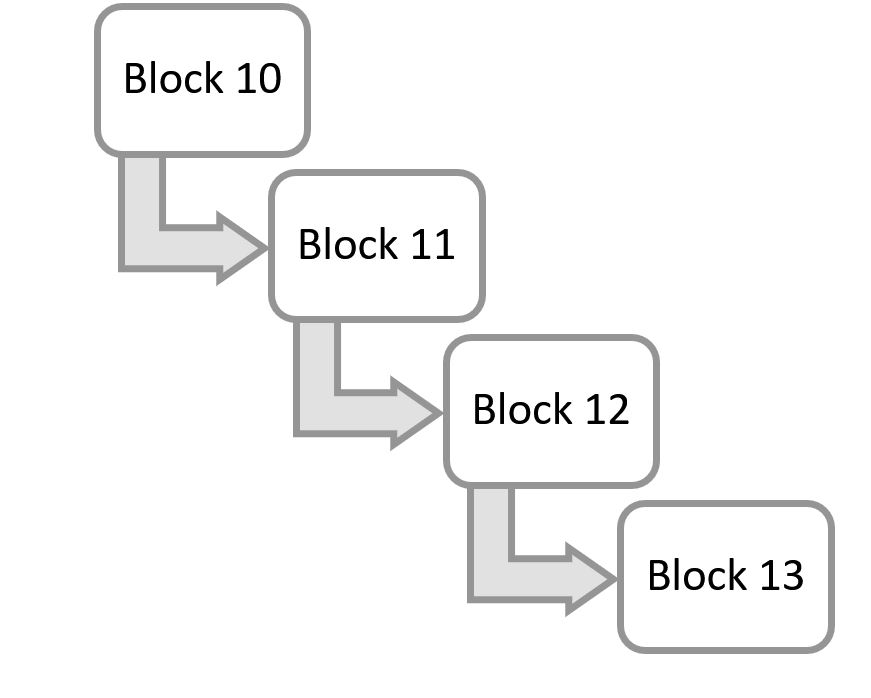
\includegraphics[scale=0.4]{pics/Block.JPG}

\end{figure}

\vspace{5mm}
To grow this chain, a block has to be added to its end. The latest one added would contain the latest transactions that have occurred using this cryptocurrency. Nodes which add a block to the blockchain would have to prove that it has done \textbf{work} by solving a hashing puzzle, which on completion would yield that node the \textbf{transaction fees} as well as a default base pay, in bitcoins. This base pay introduces new bitcoins into the network and is the only source of generation of these coins, barring the first initial block, termed as the \textbf{genesis block}.
\vspace{10mm}
Bitcoins can be obtained in exchange for other currencies, products, and services. or users can buy, send, and receive bitcoins electronically for a nominal fee using wallet software on their a personal computer, mobile device, or a web application.
Thus it can be used as a full fledged medium of monetary exchange between individuals. Since no country owns it, it is resilient to the economic conditions of many countries around the globe.

\newpage
\begin{center}\underline{  \Large\textbf{CHAPTER2}}\end{center}
\begin{center}\underline{ \Large \textbf{HISTORY}}\end{center}


\vspace{10mm}
In 2008, a paper surfaced on the internet by an anonymous Satoshi Nakamoto, which people believe can be accredited to the 2008 US financial crisis. An exploit to create many bitcoins did occur in 2009, which was promptly fixed and was the last known major fault in this system till date. Bitcoin's worth in physical currency has been fluctuating since its inception and has since gone numerous cycles of appreciation and depreciation.
Due to this, it has been thought of by some as the next gold revolution, and by others, nothing more than just a bubble of inflation which could burst anytime.
\vspace{5mm}

In 2013, bitcoin found use in transactions over some mainstream websites. WordPress started in November 2012 followed by OKCupid in April 2013, for example.
With the sudden popularity of this currency, its value rose as more and more people wanted to trade with it and in 2013, for the first time, it crossed USD 1000 and never came back down, ever since. The year 2017 saw its price rise to 5000, and then in November that year, all the way to USD 18000. It did fall in the coming months and has been hovering around the USD 10000 mark.


\begin{figure}[h]
\centering
\caption{The price of Bitcoin in USD, over the years}
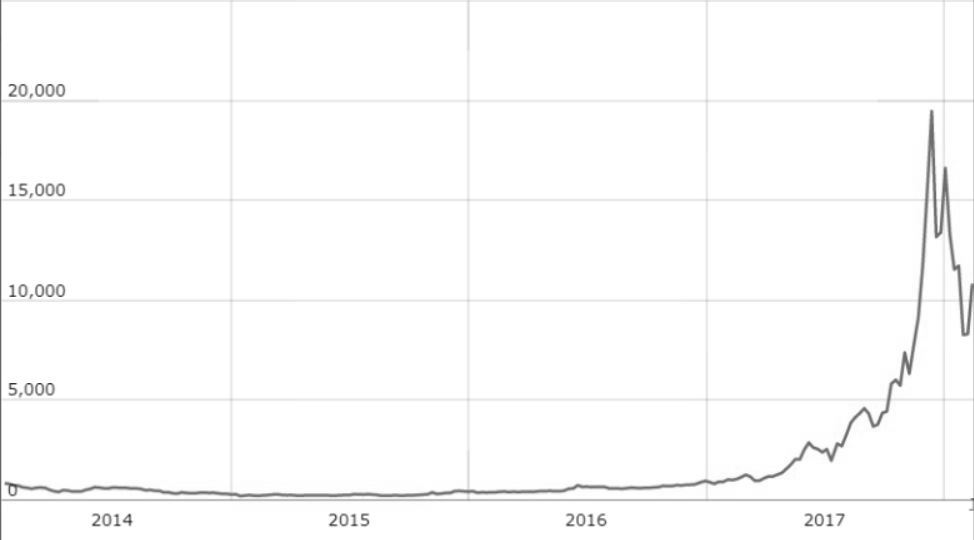
\includegraphics[scale=0.4]{pics/Price.JPG}
\end{figure}

\vspace{10mm}
Being open source, the community has grown exponentially since 2009 with many developers working on Bitcoin and ways to improve it. As its founder Satoshi Nakamoto has been anonymous ever since, some people have raised concerns over this system, many linked to the open source nature of this cryptocurrency many.

As the source code and implementation is open and freely available, anyone can participate in this decentralised system. And just as how like current developers do not control or regulate bitcoin, even its founder Satoshi had no influence over it since its inception.

\newpage
 
\begin{center}\underline{  \Large\textbf{CHAPTER 3}}\end{center}
\begin{center}\underline{ \Large \textbf{MOTIVES AND BENEFITS}}\end{center}

\vspace{10mm}
\textbf{3.1 The Reasons For Bitcoin}
\vspace{10mm}

As discussed earlier, the 2008 financial crisis was one of the leading reasons for the creation of the bitcoin. 
To summarise, the financial crisis of 2008 in the US was caused by banks which lent out risky loans to attract new customers, which would enable banks to get money to give more loans and so on. This was like a bubble, and eventually it burst in 2008. As the loans were risky, many banks were not paid back and the list of loan defaulters gradually increased. This made many banks collapse and file for bankruptcy. In addition to giving out risky loans, these banks also used people’s money to invest in various opportunities, which didn't work as intended, causing a further downfall.
\vspace{10mm}
People had trusted these banks to keep money safe, but in turn they lost it all. Noticing this widespread bankruptcy, the American Government tried saving these banks. They attempted a bail out by repaying people's money. These funds came from the taxes that were payed and it caused an overall fall in the development of the nation.
Here lies the first problem. Financial institutions do not keep people's money idly sitting. It is used to lend loans and offer other services, which could lead to a collapse like this.
Another widespread issue is that when governments overspend and are out of funds, they request banks to print more money, which in turn just devalues the currency as more of it is available.
\vspace{10mm}

Bitcoin solves these issues by account of it being a decentralised financial system. Nobody owns or regulates the money, and every transaction is accounted for.  These coins either are spent, or stay put. Not moving anywhere.

\newpage
\vspace{10mm}
\textbf{3.2 The Benefits of Bitcoin}
\vspace{10mm}

By decentralising and distributing the monetary powers of a financial institution, bitcoin can leverage consensus to make decisions. This means that nobody would tend to make risky decisions and that leads to some interesting implications, such as:

\begin{itemize}

 \item \textbf{Fewer risks} \newline People buying things using Bitcoin need not share too much information about themselves like their bank account details, names or addresses. This is a desirable aspect as people are vulnerable to attacks if their identity and bank statements are known. \newline 
 The latter isn't too hard  to obtain, if the attacker is willing enough.
 Sellers of goods and services are also benefited as these transactions are secure, irreversible, and only work if the customer has enough funds in the first place, leading to no such thing as cheque bounces. This also protects merchants from losses occurring via fraud or fraudulent chargebacks.
  
  \vspace{10mm}
  \item \textbf{Payment freedom} \newline
  As Bitcoin ensures that the maximum funds that go out of an address is available in the first place, people could buy anything at any price, without worrying too much about processing time and checks that happen in banks. Also since the internet is up and running 24/7 people are allowed to pay anytime, anywhere, not looking out for things like bank holidays. No borders. No imposed limits. Bitcoin enables its users to be in full control of their money.
  \vspace{10mm}

 \item \textbf{Transparency and neutrality} \newline 
 Every single bitcoin and fractional values of it are freely available to account for and see for any an everyone, in real time. As anybody can view it, even people who do not participate in bitcoin transactions can do this too. Rest assured that the identities of the transacting parties would never be known.\newline
 Neutrality is ensured as no individual or organisation can control or manipulate the Bitcoin protocol because as it is cryptographically secure. This allows the core of Bitcoin to be trusted for being completely neutral, transparent and predictable.
 
  \vspace{10mm}
 
  
  \item \textbf{Low fees} \newline 
  Currently, there are zero transaction fees, if the user isn't in an imminent situation to have their transaction verified. Users include fees with transactions if they want to receive priority processing, resulting in faster confirmation of transactions. This allows for a market of merchant processors to assist in processing transactions by converting bitcoins to fiat currency and depositing funds directly into merchants' bank accounts daily. As these services are based on Bitcoin, they can be offered for much lower fees than with PayPal or credit card networks
  
  \vspace{10mm}
  
  \item \textbf{Control and Security} \newline 
  The only person authorised to move money out of an address is the one who holds the account information only. Thus, any merchant has no way to to force unwanted or unnoticed charges, which is common practise in today's institutional banking services. This offers strong protection against identity theft. Also, if desired, Bitcoin users can also protect their money with backup and encryption.
  

\end{itemize}


\newpage

\begin{center}\underline{  \Large\textbf{CHAPTER 4}}\end{center}
\begin{center}\underline{ \Large \textbf{Digital Currency}}\end{center}

\vspace{10mm}

To fully appreciate the development of the Bitcoin protocol, it would be desirable to look at the inherent difficulties that one would face, if they attempt to build such a system on their own. Starting from the most fundamental issues and then building up on it, we can understand why the protocol does what it does.
\vspace{10mm}

\textbf{4.1 Currency in a Computer Hard Disk}

\begin{center}\includegraphics[width=7cm]{download1}\end{center}
\begin{center}\textbf{Fig 3.3 Scales per Octave}\end{center}
\vspace{10mm}

Fig 3.3 shows the simulation results used to verify the effect of different   number of scales per octave at which the image function is sampled preceding to extrema detection. In this case, each image was resampled following rotation by some random angle and scaling randomly  in  between 0.2 of 0.9 times the original image size. Key points from the reduced resolution image were matched against those from the original image.\par

\vspace{10mm}
The top line in fig 3.3 shows  the percentage of key points that  detected the  matching location and scale in the transformed image. Here , we define matching scale as approximate within a factor of $\sqrt{2}$. The correct scale, and a matching location as being within $\sigma$ pixels, where  is the scale of the key point . The lower line on this graph shows the number of key points that are correctly matched to a database of 40,000 key points using the nearest-neighbor matching (this shows that once a  key point is repeatability  located, it is useful to use it for  recognition and matching tasks). As fig3.3 shows, the highest repeatability is obtained when sampling 3 scales per octave, and this is the number of scale we have used for determination of features.\par
\vspace{10mm}
\begin{center}\includegraphics[width=15em]{bharat1}\end{center}

\begin{center}\textbf{Fig 3.4 Number of scales for  calculating DOG}\end{center}

\vspace{10mm}

It is surprising that as we increase the number of scale per octave the repeatability doesn't improve. This is due to the fact that as we increase the number of scales many more local extrema will be detected which are unstable and have low contrast, as  shown in fig 3.4 
This figure shows the average number key points correctly detected in  each image.\par
\vspace{10mm}

The number of keypoints increases with increased sampling of scales and the total number of correct matches also rises. Since the success of object recognition often depends more on the quantity of correctly matched keypoints, as opposed to their percentage correct matching, for many applications it will be optimal to use a larger number of scale samples. However, the cost of computation rises with increase of scale, so we should preferably  choose to use just 3 scale samples per octave.\par

\vspace{10mm}
To summarize, these experimentshave shown us that scale-space difference-of-Gaussian function have many number of extrema and  it would be expensive to detect them all. Fortunately, we can detect the most stable subset even with a coarse sampling of scales.\par

\newpage



\textbf{3.3 Sampling  in spatial domain}
\vspace{10mm}

As in the previous section we determined the sampling frequency required per octave of scale space, now we should  determine the frequency of sampling in the image domain relative to the scale of smoothing($\sigma$). As the extrema can be arbitrarily really close together, there is a trade-off between sampling frequency and rate of detection. Figure 3.5 shows an experimental determination of the amount of prior smoothing, $\sigma$, that is applied to each image initially. The top line is the repeatability of keypoint detection, and the results show that the repeatability continuously increases with $ \sigma$ . The cost increases with  $\sigma$ in terms of efficiency, so we have choose to use  $\sigma$= 1.6, which provides close to optimal repeatability. This value is used for calculating keypoints and  results is shown in  Fig 3.5


\vspace{10mm}

\begin{center}\includegraphics[width=12cm]{ert}\end{center}
\begin{center}\textbf{Fig 3.5 Sampling in Spatial domain}\end{center}

\newpage





\begin{center}\underline{ \Large \textbf{CHAPTER4}}\end{center}
\begin{center}\underline{ \Large \textbf{ACCURATE KEYPOINT LOCALIZATION}}\end{center}
\vspace{10mm}


\textbf{4.1 Initial Outlier Rejection}

\vspace{10mm}

After a keypoint candidate has been detected by comparing a pixel to its neighbors, then
we  perform a detailed fit to the nearby data for location, scale, and ratio of principal curvatures. This also helps us to  allows points to be rejected that have low contrast (and are therefore sensitive to noise) or poorly localized along an edge.\par

\vspace{10mm}



Initially we simply locate keypoints at the location and scale of the central sample point. However, Brown developed  a method for fitting a 3D quadratic function to the local sample points to determine the location of the maximum and minimum ,this turns out to have improved image matching and stability. This approach uses  Taylor expansion (up to the quadratic terms) of the scale-space function, $D(x, y, \sigma)$, shifted so that the origin is at the sample point:\par

\vspace{10mm}

\begin{center}$D(x) = D+ \frac{\partial D^T}{\partial x} +\frac{1}{2} x^T \frac{\partial^2 Dx}{\partial x^2}x\hspace{1cm}(1)$ \end{center}

\vspace{10mm}


where D and its derivatives are evaluated at the sample point and x = $(x, y,\sigma)^T$ is the offset from this point. The location of the extremum, \^x , is calculated by taking the derivative of this function with respect to x and equating  it to zero, which gives\par

\vspace{10mm}

\begin{center}$ \hat x = \frac{\partial^2 D^-1}{\partial x^2}*\frac{\partial d}{\partial x}\hspace{1cm}(2)             $\end{center} 
\vspace{10mm}


Derivative of D are estimated by calculating differences of neighboring sample points. The resulting 3x3 linear system can be solved with minimum cost. If the offset \^x is larger than 0.5 , then it means that the extremum lies closer to a different sample point. In this situation, the sample point is changed and then the interpolation is performed  about that point. The final offset \^x  is added to the location of its sample point to get the interpolated estimate for the location of the extremum. \par
\vspace{10mm}






\begin{center}\includegraphics[width=12cm]{keypoint}\end{center}
\begin{center}\textbf{Fig 4.1 Key point Localization}\end{center}


\vspace{10mm}

The function value at the extremum, D(\^x), is useful for rejecting unstable keypoint with low contrast. This can be obtained by substituting equation (2) into (1), giving

\vspace{10mm}


\begin{center}$D(\hat x) = D + \frac{1}{2}\frac{\partial D^T}{\partial \hat x}$\end{center}

\vspace{10mm}


To remove the low contrast keypoints , all extrema with a value of |D(x ̂)| less than 0.03 were discarded.
Figure 5 shows the effects of keypoint selection on a natural image. In order to avoid too
much clutter, a low-resolution 233 by 189 pixel image is used and keypoints are shown as
vectors giving the location, scale, and orientation of each keypoint (orientation assignment is described below)\par

\vspace{10mm}

Fig 4.1 shows the original image, which is shown at reduced contrast behind the subsequent figures. Fig 4.2 shows the 832 keypoints at all detected maxima and minima of the difference-of-Gaussian function, while  Fig 4.3 shows the 729 keypoints that remain following removal of those with a value of |D(x ̂)| less than 0.03. Fig 4.4 will be explained in the next section.

\newpage



\textbf{4.2 Further  Outlier Rejection}
\vspace{10mm}

In the previous section we rejected low contrast extrema from image, but it is not sufficient for stability. The DOG has a strong response  along  edges, even if the location around each edge is unstable and therefore makes small amount of noise\par

\vspace{10mm}


 DOG function with a  poor peak  will have a large \textit{principal curvature} across the edge but a small one in the perpendicular direction. Therefore  principal curvatures is  computed from a 2x2 Hessian matrix, H, computed at the location and scale of the keypoint:\par

\vspace{10mm}


\quad
\begin{center}H = $\begin{bmatrix} Dxx  & Dxy  \\ Dxy & Dyy \end{bmatrix}$\end{center}
\vspace{10mm}

The derivatives are estimated by taking differences of neighbouring sample points.

\vspace{5mm}
The eigenvalues of H are proportional to the principal curvatures of D. we can avoid explicitly computing the eigenvalues, as we are only concerned with their ratio. Let $\alpha$ be the eigenvalue with the largest magnitude and  $\beta$ be the smaller one. Then, we can compute the sum of the eigenvalues from the trace of H and their product from the determinant:
\vspace{10mm}


\begin{center}$
		Tr(H) = Dxx + Dyy = \alpha + \beta$\end{center}
		
		\vspace{1mm}
\begin{center}$		 Det(H) = Dxx*Dyy- (Dxy)^2 = \alpha*\beta$\end{center}

\vspace{10mm}

If the determinant is negative, the curvatures have different signs so the point is not  taken as an extremum. Let r be the ratio between the largest magnitude eigenvalue and the smaller one, so that $\alpha = r\beta$. Then,
		
\vspace{10mm}

\begin{center}$ \frac{Tr(H)^2}{Det(H)} = \frac{(\alpha + \beta)^2}{\alpha\beta} = \frac{r\beta + \beta}{r\beta^2} = \frac{(r+1)^2}{r},$\end{center}

\vspace{10mm}

Here the ratio only depends on  the eigenvalues rather than their individual values. The quantity$ (r+1)^2/r $ is minimum when the two eigenvalues $\alpha and \beta$  are equal and the ratio  increases with r. Therefore, to check that the ratio of principal curvatures is below some threshold, r, we only need to check if

\vspace{10mm}

\begin{center}$ \frac{Tr(H)^2}{Det(H)} <  \frac{(r+1)^2}{r},$\end{center}

\vspace{10mm}

The above algorithm is very efficient as it compute, with less than 20 floating point operations required to
test each keypoint. we eliminates keypoints that have a ratio between the principal curvatures greater than 10. The transition from Fig4.1(c) to 4.1(d) shows the effects of this operation.

\newpage




\begin{center}\underline{ \Large \textbf{CHAPTER5}}\end{center}
\begin{center}\underline{ \Large \textbf{ORIENTATION ASSIGNMENT}}\end{center}
\vspace{10mm}





Orientation assignment is done in order to  achieve rotation invariance . The scale of the keypoint
is used to select the Gaussian smoothed image, L, with the closest scale, so that  computations are executed in a scale-invariant manner.For each image sample, L(x, y) , the gradient magnitude, m(x , y), and orientation,$ \theta(x , y)$, is precomputed using pixel differences:\par


\vspace{10mm}


$m(x,y) = \sqrt{(L(x+1,y) - L(x-1,y))^2 + (L(x,y+1) - L(x,y-1))^2}$
\vspace{2mm}


$
\theta(x,y) = \tan^-1((L(x,y+1) - L(x,y-1))/(L(x+1,y) - L(x-1,y)))$


\vspace{9mm}


After computations orientation histogram is formed using the gradient orientations of sample points around the key point. The  histogram has 36 bins covering the 360 degree range of orientations. Each sample added to the histogram is weighted by its gradient magnitude and by a Gaussian-weighted circular window with a $\sigma$ that is 1.5 times that of the scale of the keypoint.\par

\vspace{10mm}




\begin{center}\includegraphics[width=12cm]{Screenshot}\end{center}
\begin{center}\textbf{Fig 5.1 Orientation Histogram}\end{center}







Peaks are generated in histogram which corresponds  to the  dominant directions of local gradients.
The highest peak in histogram  is detected, and if there is any local peak that is in the range of 
80 percentage of the highest peak is  also  used to create a keypoint with that orientation. Therefore,
locations with multiple peaks with similar magnitude will have multiple  key points created at
the same location and scale but with different orientations. Only about 15 percenatge of points are assigned
multiple orientations,these contribute significantly to the stability of matching key points. Finally, a
parabola is fit to the 3 histogram values closest to each peak to interpolate the peak position
for better accuracy.


\newpage

\begin{center}\underline{ \Large \textbf{CHAPTER6}}\end{center}
\begin{center}\underline{ \Large \textbf{LOCAL IMAGE DESCRIPTOR}}\end{center}

\vspace{10mm}





In previous section we have assigned an image location, scale, and orientation to each keypoint. These parameters create a repeatable local 2D coordinate system which  describe the local image region, and therefore provide invariance to these parameters. Now in this section we compute a descriptor for the local image region that is highly distinctive yet is as invariant as possible to remaining variations, such as change in illumination or 3D viewpoint.\par

\vspace{10 mm}

One of the approach would be to sample the local image intensities around the keypoint
at the appropriate scale, and to match these using a normalized correlation measure.
However, simple correlation of image patches is highly sensitive to changes that cause misregistration of samples, such as affine or 3D viewpoint change or non-rigid deformations.\par



\newpage


\textbf{6.1  Extraction Of Local Image Descriptor at Key Points}
\vspace{7mm}

Fig 6.1 illustrates the computation of the key point descriptor. First the image gradient magnitudes and orientations are sampled around the key point location, using the scale of the key point to select the level of Gaussian blur. In order to achieve orientation invariance, the coordinates of the descriptor and the gradient orientations are rotated relative to the key point orientation. For efficiency, the gradients are pre computed for all levels of the pyramid as described in chapter 5. These are illustrated with small arrows at each sample location on the left side of Fig 6.1.\par
\vspace{7mm}
\includegraphics{main}
\begin{center}\textbf{Fig 6.1 key point descriptor }\end{center}
\vspace{7 mm}


A Gaussian weighting function with  σ  equal to one half the width of the descriptor window is used to assign a weight to the magnitude of each sample point. This is illustrated with a circular window on the left side of Figure 6.1, although, the weight falls off smoothly. The purpose of this Gaussian window is to avoid sudden changes in the descriptor with small changes in the position of the window, and to give less emphasis to gradients that are far from the center of the descriptor, as these are most affected by errors

\newpage


The key point descriptor is shown on the right side of Figure 6.1. It allows for significant
shift in gradient positions by creating orientation histograms over 4x4 sample regions. The figure shows eight directions for each orientation histogram, with the length of each arrow corresponding to the magnitude of that histogram entry. A gradient sample on the left can shift up to 4 sample positions while still contributing to the same histogram on the right, thereby achieving the objective of allowing for larger local positional shifts\par
\vspace{7 mm}
The descriptor is formed from a vector containing the values of all the orientation histogram entries, corresponding to the lengths of the arrows on the right side of Figure 7. The figure shows a 2x2 array of orientation histograms, whereas our experiments below show that the best results are achieved with a 4x4 array of histograms with 8 orientation bins in each. Therefore, the experiments in this paper use a 4x4x8 = 128 element feature vector for each key point.\par

\vspace{7 mm}


\textbf{6.1.1  Remove illumination effect}\\
 To reduce the effects of illumination we need to normalize the feature vector to unit length. A change in image contrast in which each pixel value is multiplied by a constant will multiply gradients by the same constant, so this contrast change will be canceled by vector normalization. A brightness change in which a constant is added to each image pixel will not affect the gradient values, as they are computed from pixel differences. Therefore, the descriptor is invariant to affine changes in illumination\par




\vspace{7mm}
However, non-linear illumination changes can also occur due to camera saturation or due to illumination changes that affect 3D surfaces with differing orientations by different amounts. These effects can cause a large change in relative magnitudes for some gradients, but are less likely to affect the gradient orientations. Therefore, we reduce the influence of large gradient magnitudes by thresholding the values in the unit feature vector to each be no larger than 0.2, and then renormalizing to unit length. the distribution of orientations has greater emphasis.




\newpage



\textbf{6.2  Descriptor Testing}


Two parameters  can be used to vary the complexity of the descriptor: the
number of orientations, r, in the histograms, and the width, n, of the nxn array of orientation
histograms. The size of the resulting descriptor vector is $rn^2$. As the complexity increases, it will be able to discriminate better in a large database, but it will also be
more sensitive to shape distortions and occlusion.\par
\vspace{10 mm}
\begin{center}\includegraphics[width = 10cm]{slide}\end{center}
\begin{center}
\textbf{Fig 6.2 Optimum width for Descriptor}
\end{center}

\vspace{10mm}

Figure 6.2 shows experimental results in which the number of orientations and size of the
descriptor were varied. The graph was generated for a viewpoint transformation in which a
planar surface is tilted by 50 degrees away from the viewer and 4 per of noise.\par
\vspace{10mm}
The results
continue to improve up to a 4x4 array of histograms with 8 orientations. After that, adding
more orientations or a larger descriptor can actually hurt matching by making the descriptor
more sensitive to distortion.







\newpage
\begin{center}\underline{ \Large \textbf{CHAPTER7}}\end{center}
\begin{center}\underline{ \Large \textbf{CONCLUSION}}\end{center}
\vspace{10mm}





The SIFT keypoints are particularly important  due to their distinctiveness,
which enables them to get correct match for a keypoint which is selected from a large database of
other keypoints. The distinctiveness of keypoints are achieved by representing the image gradients with  high-dimensional vector within a local region of the image. The keypoints are
shown to be invariant to image rotation , scale ,  affine distortion, addition of noise, and change in illumination. Large numbers of keypoints can be extracted from  images, which leads to robustness in extracting small objects
among noise.Keypoints are detected over a complete range of scales determines that the 
small local features are available for matching small , while large
keypoints perform well for images subject to noise ,blur and clutter. The computation is efficient,
as several thousand keypoints can be extracted from a typical image with near real-time
performance on standard PC hardware.








\newpage

\begin{center}\underline{ \Large \textbf{REFERENCES}}\end{center}

[1]Witkin, A.P. 1983. Scale-space filtering. In International Joint Conference on Artificial Intelligence,
Karlsruhe, Germany, pp. 1019-1022.\\

[2] Mikolajczyk, K., and Schmid, C. 2002. An affine invariant interest point detector. In European
Conference on Computer Vision (ECCV), Copenhagen, Denmark, pp. 128-142.\\

[3]Lindeberg, T. 1993. Detecting salient blob-like image structures and their scales with a scale-space
primal sketch: a method for focus-of-attention. International Journal of Computer Vision, 11(3):
283-318.

[4]Lowe, D.G. 2001. Local feature view clustering for 3D object recognition. IEEE Conference on
Computer Vision and Pattern Recognition, Kauai, Hawaii, pp. 682-688.\\

[5]Harris, C. and Stephens, M. 1988. A combined corner and edge detector. In Fourth Alvey Vision
Conference, Manchester, UK, pp. 147-151.\\

[6]Brown, M. and Lowe, D.G. 2002. Invariant features from interest point groups. In British Machine
Vision Conference, Cardiff, Wales, pp. 656-665.\\

[7]https://www.youtube.com/watch?v=NPcMS49V5hg






 \end{flushleft}



\end{document}

